\documentclass{beamer}

\usepackage{amsmath}
\usepackage{amssymb}
\usepackage{booktabs}
\usepackage{tabularx}

\usetheme{Madrid}
\usecolortheme{beaver}
\usepackage[utf8]{inputenc}
\usepackage[brazil]{babel}
\usepackage{graphicx}
\usepackage{xcolor}
\usepackage{colortbl}
\usepackage{tikz}
\usetikzlibrary{shapes.geometric, arrows.meta, positioning, calc, decorations.pathreplacing}
\usepackage{array}
\usepackage{tcolorbox}
\tcbuselibrary{skins, breakable}
\usepackage{hyperref}
\hypersetup{
    colorlinks=true,
    filecolor=magenta,
    urlcolor=cyan,
    pdfpagemode=FullScreen,
    }
\urlstyle{same}

\definecolor{graycell}{gray}{0.85}
\definecolor{vermelhoClaro}{RGB}{255, 200, 200}

\AtBeginSection[]
{
  \begin{frame}
    \frametitle{Índice}
    \tableofcontents[currentsection]
  \end{frame}
}

%%%%%%%%%%%%%%%%%%%%%%%%%%%%%%%%%%%%%%%%%%%%%%%%%%%%%%%%%%%%%%%%%%%%%
%% Estilos para diagramas de protocolo (message sequence charts)
%% (mesmos estilos das aulas de Kerberos e PKI)
%%%%%%%%%%%%%%%%%%%%%%%%%%%%%%%%%%%%%%%%%%%%%%%%%%%%%%%%%%%%%%%%%%%%%
\tikzset{
    ator/.style   = {font=\footnotesize\bfseries},
    chave/.style  = {font=\scriptsize\itshape, text=black!55},
    vida/.style   = {gray!55, dashed, thick},
    msg/.style    = {-{Latex[length=2mm]}, thick, blue!55!black},
    comp/.style   = {font=\scriptsize, draw=black!25, fill=black!4, rounded corners,
                     inner sep=2.5pt, align=left},
    rotmsg/.style = {font=\scriptsize, fill=white, inner sep=1.5pt},
}

%%%%%%%%%%%%%%%%%%%%%%%%%%%%%%%%%%%%%%%%%%%%%%%%%%%%%%%%%%%%%%%%%%%%%
%% Estilos para árvores (Merkle) e blocos (McEliece / famílias)
%%%%%%%%%%%%%%%%%%%%%%%%%%%%%%%%%%%%%%%%%%%%%%%%%%%%%%%%%%%%%%%%%%%%%
\tikzset{
    noh/.style    = {draw=blue!55!black, fill=blue!8, rounded corners, thick,
                     font=\scriptsize\bfseries, align=center, inner sep=3pt, minimum width=1.0cm},
    raiz/.style   = {draw=green!50!black, fill=green!10, rounded corners, thick,
                     font=\scriptsize\bfseries, align=center, inner sep=3.5pt, minimum width=1.1cm},
    folha/.style  = {draw=orange!70!black, fill=orange!10, rounded corners,
                     font=\tiny, align=center, inner sep=2.5pt, minimum width=0.8cm},
    bloco/.style  = {draw=black!40, fill=black!4, rounded corners, thick,
                     font=\scriptsize, align=center, inner sep=4pt},
    lig/.style    = {-{Latex[length=1.6mm]}, thick, black!55},
}

% Título da apresentação
\title[Criptografia Pós-Quântica]{Introdução à Criptografia Pós-Quântica}
\author{Prof. Iaçanã Ianiski Weber}
\institute{PUCRS}
\date{CSS (98G08-4)}

\begin{document}

% Slide de Capa
\begin{frame}[plain]
\noindent
\begin{minipage}[t]{0.15\textwidth}
    
\includegraphics[width=\linewidth]{img/Brasão_PUCRS.png}
\end{minipage}%
\begin{minipage}[t]{0.84\textwidth}
    \begin{center}
        {\LARGE\bfseries\textcolor{blue}{Introdução à\\[2pt] Criptografia Pós-Quântica}}
    \end{center}
\end{minipage}

\vspace{1.6cm}

\begin{center}
    \Large \textbf{Prof. Dr. Iaçanã Ianiski Weber} \\
    \vspace{0.2cm}
    \normalsize \textit{Confiabilidade e Segurança de Software} \\
    \vspace{0.2cm}
    \large 98G08-4
\end{center}

\vfill

\begin{center}
    \tiny \textit{Agradecimentos especiais ao Prof. Avelino Zorzo e aos Autores Christof Paar, Jan Pelzl e Tim Güneysu pelo material (cap.\ 12). Padrões e prazos baseados em publicações do NIST, NSA, BSI, ANSSI, NCSC e demais agências.}
\end{center}
\end{frame}

% Índice
\begin{frame}{Índice}
    \tableofcontents
\end{frame}

\begin{frame}{Conteúdo desta Aula}
    \vspace{0.3em}
    Nesta aula você vai entender:
    \begin{itemize}
        \item Por que o computador quântico ameaça a criptografia atual, e o que os algoritmos de \textbf{Shor} e \textbf{Grover} de fato quebram.
        \medskip
        \item O que é (e o que não é) a \textbf{Criptografia Pós-Quântica (PQC)}, e por que ``colher agora, decifrar depois'' torna o problema urgente.
        \medskip
        \item As três famílias principais (reticulados, códigos e hash), com a intuição de cada uma e seus compromissos de tamanho e desempenho.
        \medskip
        \item Os padrões do \textbf{NIST} de 2024 (ML-KEM, ML-DSA, SLH-DSA) e como surgiram.
        \medskip
        \item Como EUA, União Europeia, Reino Unido, China e Rússia estão conduzindo a transição, e por que isso importa.
        \medskip
        \item A estratégia de migração híbrida já em uso na prática, como no TLS 1.3.
    \end{itemize}
\end{frame}

\begin{frame}{A Criptografia de Chave Pública Sob Ameaça}
    Ao longo do curso, a criptografia de chave pública apoiou-se em dois problemas ``difíceis'':
    \begin{itemize}
        \footnotesize
        \item \textbf{Fatoração de inteiros}, que sustenta o \textbf{RSA}.
        \item \textbf{Logaritmo discreto} (em $\mathbb{Z}_p^*$ ou em curvas elípticas), que sustenta \textbf{Diffie--Hellman}, \textbf{ECDH} e \textbf{ECDSA}.
    \end{itemize}
    \medskip
    \begin{tcolorbox}[colback=red!5,colframe=red!60!black,boxrule=0.5pt]
        \footnotesize
        Esses problemas são difíceis para computadores clássicos, mas não para um computador \textbf{quântico} suficientemente grande. Um único algoritmo, o de \textbf{Shor}, derruba RSA, DH e ECC.
    \end{tcolorbox}
    \medskip
    \begin{itemize}
        \footnotesize
        \item A criptografia simétrica (AES) e as funções hash (SHA-2/3) são muito menos afetadas.
        \item O objetivo da aula é entender as alternativas assimétricas que resistem a ataques quânticos, ou seja, a Criptografia Pós-Quântica.
    \end{itemize}
    \smallskip
    {\tiny Fonte: Paar, Pelzl \& Güneysu (2024), cap.\ 12 (\textit{Post-Quantum Cryptography}), §12.1.}
\end{frame}

%%%%%%%%%%%%%%%%%%%%%%%%%%%%%%%%%%%%%%%%%%%%%%%%%%%%%%%%%%%%%%%%%%%%%
\section{A Ameaça Quântica}

\begin{frame}{Como um Computador Quântico Ataca a Criptografia}
    \begin{columns}[T]
        \begin{column}{0.56\textwidth}
            \footnotesize
            Um computador quântico não é apenas mais rápido; ele calcula de outra forma.
            \begin{itemize}
                \item \textbf{Bit} clássico: 0 ou 1.
                \item \textbf{Qubit}: em superposição de 0 e 1; $n$ qubits representam $2^n$ estados ao mesmo tempo.
                \item Emaranhamento e interferência permitem algoritmos que amplificam a resposta certa.
            \end{itemize}
            \smallskip
            Isso não quebra ``tudo''. Só ajuda em problemas com estrutura matemática explorável, como a periodicidade em que se apoiam a fatoração e o logaritmo discreto.
        \end{column}
        \begin{column}{0.42\textwidth}
            \centering
            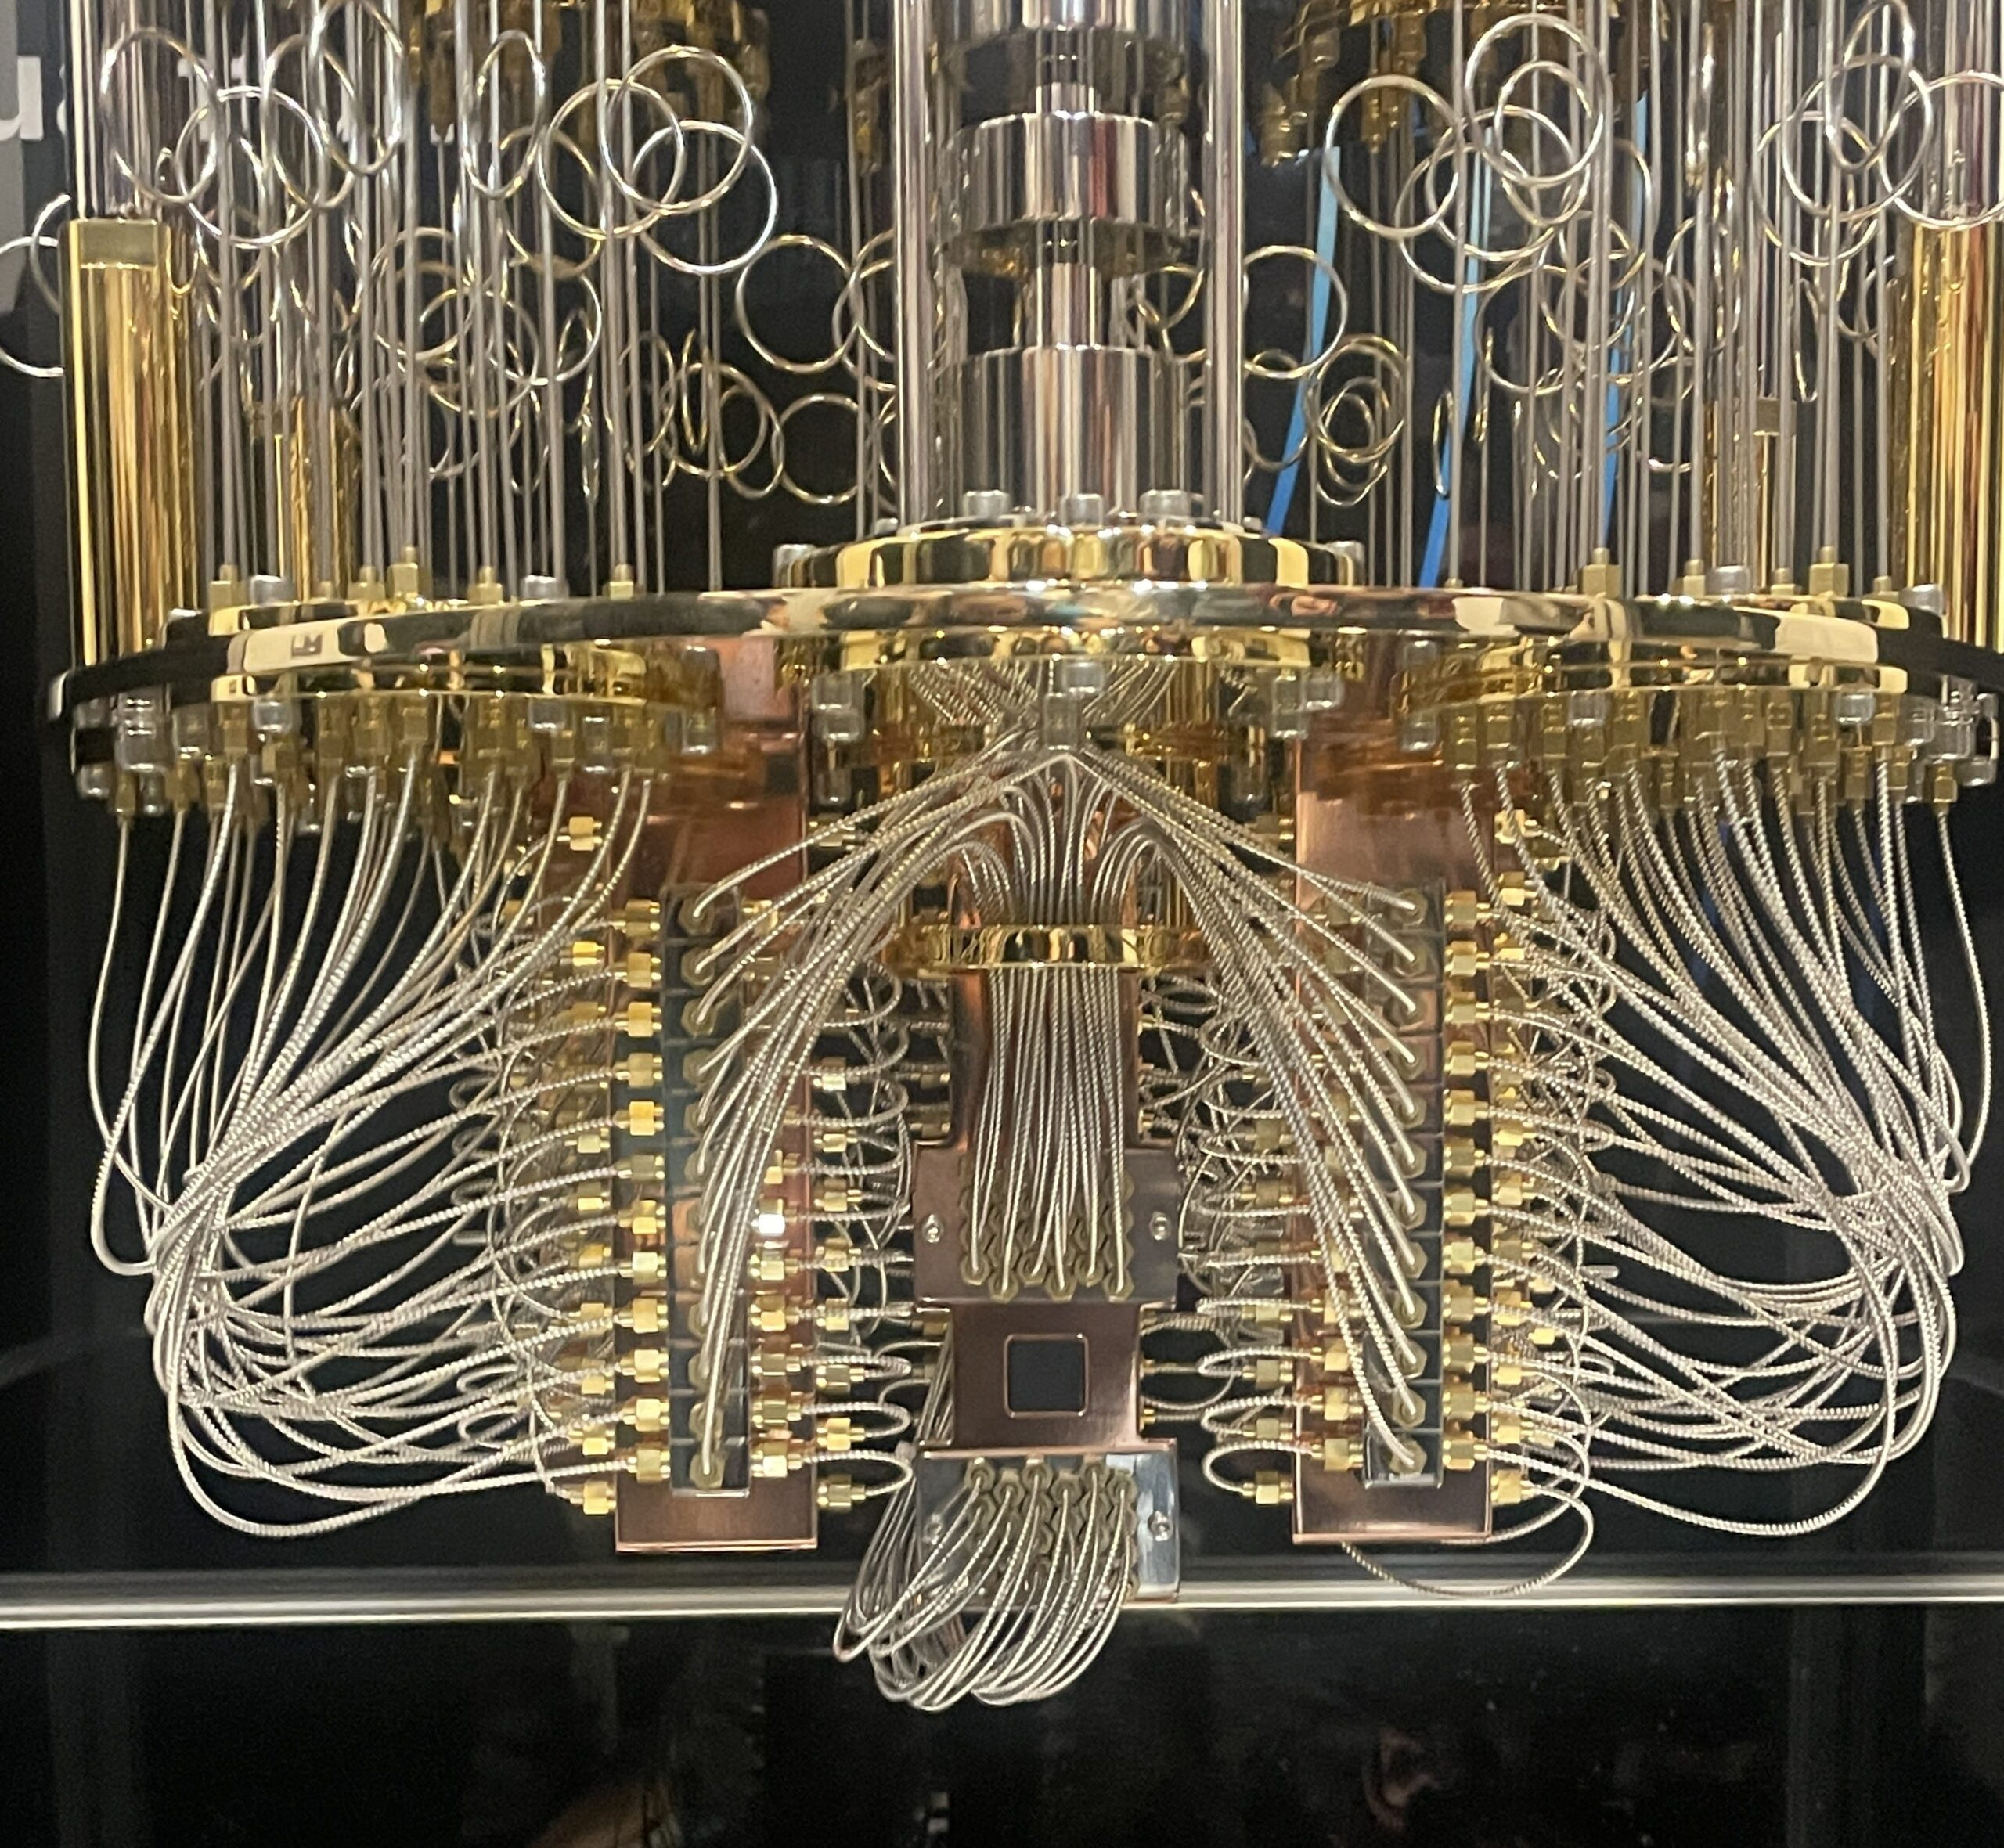
\includegraphics[width=\linewidth,height=4.1cm,keepaspectratio]{img/quantum_computer.jpeg}
            \\[2pt]{\tiny Processador quântico supercondutor no seu criostato de diluição.}
        \end{column}
    \end{columns}
    \medskip
    \begin{tcolorbox}[colback=blue!5,colframe=blue!50!black,boxrule=0.5pt]
        \footnotesize
        Dois algoritmos quânticos importam para a criptografia: \textbf{Shor} (1994) e \textbf{Grover} (1996).
    \end{tcolorbox}
\end{frame}

\begin{frame}{Algoritmo de Shor (1994)}
    \begin{tcolorbox}[colback=red!5,colframe=red!60!black,boxrule=0.5pt,title={\footnotesize O que Shor faz}]
        \footnotesize
        Resolve a \textbf{fatoração de inteiros} e o \textbf{logaritmo discreto} em tempo polinomial num computador quântico. O que era inviável (custo exponencial) passa a ser eficiente.
    \end{tcolorbox}
    \medskip
    \begin{itemize}
        \footnotesize
        \item Como consequência, \textbf{RSA}, \textbf{Diffie--Hellman}, \textbf{ECDH} e \textbf{ECDSA} tornam-se inseguros. Não adianta aumentar o tamanho da chave, pois o ataque é polinomial.
        \item Foi a descoberta de Shor que transformou a computação quântica de curiosidade teórica em ameaça concreta à segurança da informação.
        \item Falta ainda o hardware: um \textbf{CRQC} (\textit{Cryptographically Relevant Quantum Computer}) capaz de rodar Shor em chaves reais ainda não existe, mas pode vir a existir.
    \end{itemize}
    \smallskip
    {\tiny Fonte: Paar et al.\ (2024), cap.\ 12 (Prefácio/§12.1); P. Shor, ``\textit{Algorithms for quantum computation}'', 1994.\par}
    \smallskip
    {\tiny Vídeo recomendado sobre o algoritmo de Shor: \url{https://www.youtube.com/watch?v=lvTqbM5Dq4Q}\par}
\end{frame}

\begin{frame}{Algoritmo de Grover (1996)}
    \begin{tcolorbox}[colback=gray!8,colframe=gray!60!black,boxrule=0.5pt]
        \centering\footnotesize
        Grover busca em um espaço de $N$ elementos em cerca de $\sqrt{N}$ passos, um ganho quadrático (não exponencial).
    \end{tcolorbox}
    \medskip
    \begin{itemize}
        \footnotesize
        \item Contra uma cifra simétrica de chave de $k$ bits, Grover reduz a busca de $2^{k}$ para cerca de $2^{k/2}$.
        \item A solução é dobrar o parâmetro: o AES-128 cai para $\sim$64 bits de segurança efetiva, então usa-se \textbf{AES-256} (cerca de 128 bits pós-Grover, seguro).
        \item Para funções hash, o ganho vale para a pré-imagem (a segurança de $n$ cai para $n/2$ bits), o que se resolve com saídas maiores. Já a resistência a colisão é limitada pelo ataque de aniversário ($2^{n/2}$), sem ganho quântico prático.
    \end{itemize}
    \medskip
    \begin{tcolorbox}[colback=green!6,colframe=green!50!black,boxrule=0.5pt]
        \footnotesize
        Por isso o foco da PQC é a criptografia assimétrica: a simétrica e as funções hash continuam seguras apenas aumentando o tamanho de chaves e saídas.
    \end{tcolorbox}
    \smallskip
    {\tiny Vídeo recomendado sobre o algoritmo de Grover: \url{https://youtube.com/watch?v=RQWpF2Gb-gU}}
\end{frame}

\begin{frame}{Impacto Quântico por Primitiva Criptográfica}
    \begin{center}
    \renewcommand{\arraystretch}{1.3}
    \footnotesize
    \begin{tabularx}{\linewidth}{@{}l l >{\raggedright\arraybackslash}X@{}}
        \toprule
        \textbf{Primitiva} & \textbf{Ataque quântico} & \textbf{Efeito} \\
        \midrule
        \rowcolor{red!8} RSA-2048/3072 & Shor & \textbf{Quebrado} (segurança $\to 0$) \\
        \rowcolor{red!8} DH / ECDH / ECDSA & Shor & \textbf{Quebrado} (segurança $\to 0$) \\
        \midrule
        \rowcolor{green!8} AES-128 & Grover & Enfraquecido ($\sim$64 bits): migrar para AES-256 \\
        \rowcolor{green!8} AES-256 & Grover & Seguro ($\sim$128 bits efetivos) \\
        \rowcolor{green!8} SHA-256 / SHA-3 & Grover & Seguro (pré-imagem $\to n/2$; colisão inalterada) \\
        \bottomrule
    \end{tabularx}
    \end{center}
    \medskip
    \begin{tcolorbox}[colback=blue!5,colframe=blue!50!black,boxrule=0.5pt]
        \footnotesize
        \textbf{Leitura da tabela:} o problema urgente é a troca de chaves e as assinaturas (chave pública). É nesse ponto que precisamos de novos algoritmos.
    \end{tcolorbox}
    \smallskip
    {\tiny Fonte: Paar et al.\ (2024), cap.\ 12; NIST IR 8105 (\textit{Report on Post-Quantum Cryptography}).}
\end{frame}

\begin{frame}{``Colher Agora, Decifrar Depois'' (\textit{Harvest Now, Decrypt Later})}
    \begin{tcolorbox}[colback=red!5,colframe=red!60!black,boxrule=0.5pt]
        \footnotesize
        Um adversário pode gravar hoje o tráfego cifrado (e-mails, registros médicos, segredos de Estado) e decifrá-lo no futuro, quando tiver um CRQC. O ataque é passivo, indetectável e já pode estar em curso.
    \end{tcolorbox}
    \medskip
    \begin{itemize}
        \footnotesize
        \item A ameaça não espera o computador quântico chegar: dados com longo prazo de sigilo já estão em risco agora.
        \item Por isso as agências de segurança tratam a migração como prioridade imediata, mesmo sem saber a data exata do CRQC.
    \end{itemize}
    \medskip
    \begin{tcolorbox}[colback=blue!5,colframe=blue!50!black,boxrule=0.5pt]
        \footnotesize
        \textbf{Pergunta-chave:} por quantos anos os seus dados precisam permanecer secretos? Se a resposta for ``mais de 10 anos'', você já tem um problema pós-quântico.
    \end{tcolorbox}
    \smallskip
    {\tiny Fonte: NIST IR 8105; ENISA / NSA / NCSC (orientações sobre \textit{harvest now, decrypt later}).}
\end{frame}

\begin{frame}{A Desigualdade de Mosca}
    \begin{columns}[c]
        \begin{column}{0.74\textwidth}
            Michele Mosca propôs uma regra simples para decidir a urgência da migração:
        \end{column}
        \begin{column}{0.24\textwidth}
            \centering
            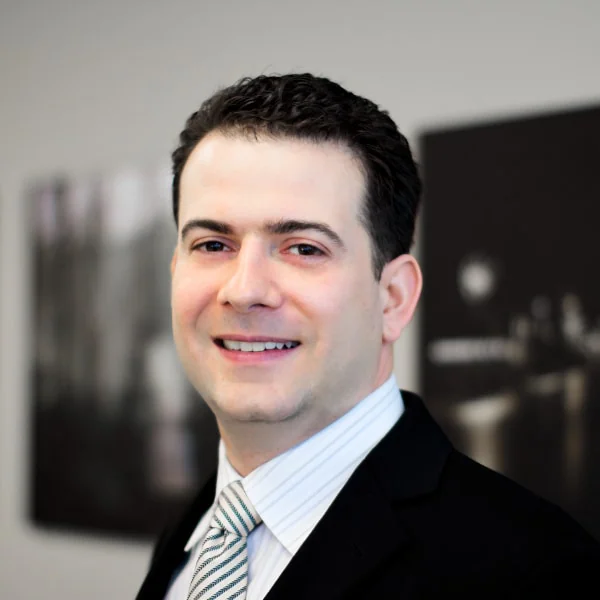
\includegraphics[width=1.7cm]{img/michele_mosca.png}\\[1pt]
            {\tiny Michele Mosca}
        \end{column}
    \end{columns}
    \vspace{0.2em}
    \begin{center}
    \resizebox{0.92\textwidth}{!}{%
    \begin{tikzpicture}[font=\footnotesize]
        % eixo do tempo
        \draw[-{Latex[length=2mm]}, thick] (0,0) -- (12,0) node[right]{tempo};
        \node[align=center, font=\scriptsize] at (0,-0.35) {hoje};
        % Z: tempo até o CRQC
        \draw[decorate, decoration={brace, amplitude=6pt}, thick, red!60!black]
            (0,2.1) -- (7.5,2.1) node[midway, above=6pt, font=\scriptsize\bfseries, text=red!60!black]{$Z$: tempo até existir um CRQC};
        \draw[red!55!black, dashed, thick] (7.5,0) -- (7.5,2.3);
        % X: shelf-life
        \fill[blue!45!black] (0,1.1) rectangle (5.5,1.5);
        \node[white, font=\scriptsize\bfseries] at (2.75,1.3) {$X$: sigilo necessário dos dados};
        % Y: migration
        \fill[orange!75!black] (5.5,1.1) rectangle (9.2,1.5);
        \node[white, font=\scriptsize\bfseries] at (7.35,1.3) {$Y$: tempo de migrar};
        % marca X+Y
        \draw[black, thick] (9.2,0.9) -- (9.2,1.7);
        \draw[decorate, decoration={brace, amplitude=6pt, mirror}, thick]
            (0,0.7) -- (9.2,0.7) node[midway, below=6pt, font=\scriptsize\bfseries]{$X + Y$};
    \end{tikzpicture}%
    }
    \end{center}
    \vspace{-0.1em}
    \begin{tcolorbox}[colback=red!5,colframe=red!60!black,boxrule=0.5pt]
        \centering\footnotesize
        Se \quad $\mathbf{X + Y > Z}$, \quad seus dados serão expostos, e já é tarde para começar a migrar.
    \end{tcolorbox}
    \smallskip
    {\tiny $X$ = anos que a informação precisa ficar secreta; $Y$ = anos para migrar os sistemas; $Z$ = anos até surgir um CRQC. Fonte: M. Mosca (2015/2018).}
\end{frame}

%%%%%%%%%%%%%%%%%%%%%%%%%%%%%%%%%%%%%%%%%%%%%%%%%%%%%%%%%%%%%%%%%%%%%
\section{O que é Criptografia Pós-Quântica}

\begin{frame}{Definição}
    \begin{block}{Criptografia Pós-Quântica (PQC)}
        \footnotesize
        Esquemas criptográficos assimétricos, executados em computadores clássicos comuns, cuja segurança se acredita resistir a ataques de computadores quânticos.
    \end{block}
    \medskip
    \begin{itemize}
        \footnotesize
        \item A ideia é substituir a fatoração e o log discreto por outros problemas difíceis, para os quais não se conhece algoritmo quântico eficiente.
        \item Não exige hardware especial: a PQC roda em notebooks, celulares e servidores de hoje. Muda apenas a matemática.
        \item As duas funções que mais precisamos substituir são o estabelecimento de chave (KEM) e a assinatura digital.
    \end{itemize}
    \medskip
    \begin{tcolorbox}[colback=gray!8,colframe=gray!60!black,boxrule=0.5pt]
        \footnotesize
        Também é chamada de criptografia ``quântico-resistente'' ou ``quantum-safe''.
    \end{tcolorbox}
    \smallskip
    {\tiny Fonte: Paar et al.\ (2024), cap.\ 12, §12.1; NIST IR 8105.}
\end{frame}

\begin{frame}{PQC Não é Criptografia Quântica (QKD)}
    \begin{columns}[T]
        \begin{column}{0.5\textwidth}
            \begin{tcolorbox}[colback=green!6,colframe=green!50!black,boxrule=0.5pt,title={\footnotesize Criptografia Pós-Quântica (PQC)}]
                \footnotesize
                \begin{itemize}
                    \item Software e matemática clássica.
                    \item Roda em qualquer computador atual.
                    \item Substitui RSA/ECC por novos problemas difíceis.
                    \item É o caminho recomendado por NIST e NSA.
                \end{itemize}
            \end{tcolorbox}
        \end{column}
        \begin{column}{0.5\textwidth}
            \begin{tcolorbox}[colback=blue!5,colframe=blue!50!black,boxrule=0.5pt,title={\footnotesize Distribuição Quântica de Chave (QKD)}]
                \footnotesize
                \begin{itemize}
                    \item Hardware quântico (fótons, fibra dedicada).
                    \item Distribui chaves usando física quântica.
                    \item Cara, com alcance limitado; não faz assinatura.
                    \item A NSA não a recomenda para sistemas nacionais.
                \end{itemize}
            \end{tcolorbox}
        \end{column}
    \end{columns}
    \medskip
    \begin{tcolorbox}[colback=red!5,colframe=red!60!black,boxrule=0.5pt]
        \footnotesize
        Não confunda as duas. Esta aula trata de \textbf{PQC} (algoritmos em software). A QKD é uma tecnologia diferente e complementar, com limitações práticas importantes.
    \end{tcolorbox}
    \smallskip
    {\tiny Fonte: NSA, ``\textit{Quantum Key Distribution (QKD) and Quantum Cryptography (QC)}'' (FAQ); NIST IR 8105.}
\end{frame}

\begin{frame}{As Famílias da Criptografia Pós-Quântica}
    \begin{center}
    \renewcommand{\arraystretch}{1.25}
    \scriptsize
    \begin{tabularx}{\linewidth}{@{}l l l >{\raggedright\arraybackslash}X@{}}
        \toprule
        \textbf{Família} & \textbf{Problema difícil} & \textbf{Serve para} & \textbf{Exemplos (padrão NIST)} \\
        \midrule
        \rowcolor{blue!7} \textbf{Reticulados} & LWE / SVP & KEM e assinatura & Kyber (\textbf{ML-KEM}), Dilithium (\textbf{ML-DSA}), Falcon \\
        \textbf{Códigos} & Decodificação de síndrome & KEM & McEliece, BIKE, \textbf{HQC} \\
        \rowcolor{green!7} \textbf{Hash} & Resistência da função hash & Assinatura & SPHINCS+ (\textbf{SLH-DSA}) \\
        \textbf{Multivariada} & Sistemas quadráticos & Assinatura & Rainbow (quebrada) \\
        \rowcolor{gray!10} \textbf{Isogenias} & Caminhos entre curvas & KEM & SIKE (quebrada em 2022) \\
        \bottomrule
    \end{tabularx}
    \end{center}
    \medskip
    \begin{itemize}
        \footnotesize
        \item Vamos estudar as três primeiras, que são as mais maduras: reticulados, códigos e hash.
        \item As duas últimas trazem uma lição importante: nem toda proposta sobrevive à criptoanálise.
    \end{itemize}
    \smallskip
    {\tiny Fonte: Paar et al.\ (2024), cap.\ 12, §§12.1--12.4.}
\end{frame}

\begin{frame}{O Custo: Chaves e Assinaturas Maiores}
    \begin{center}
        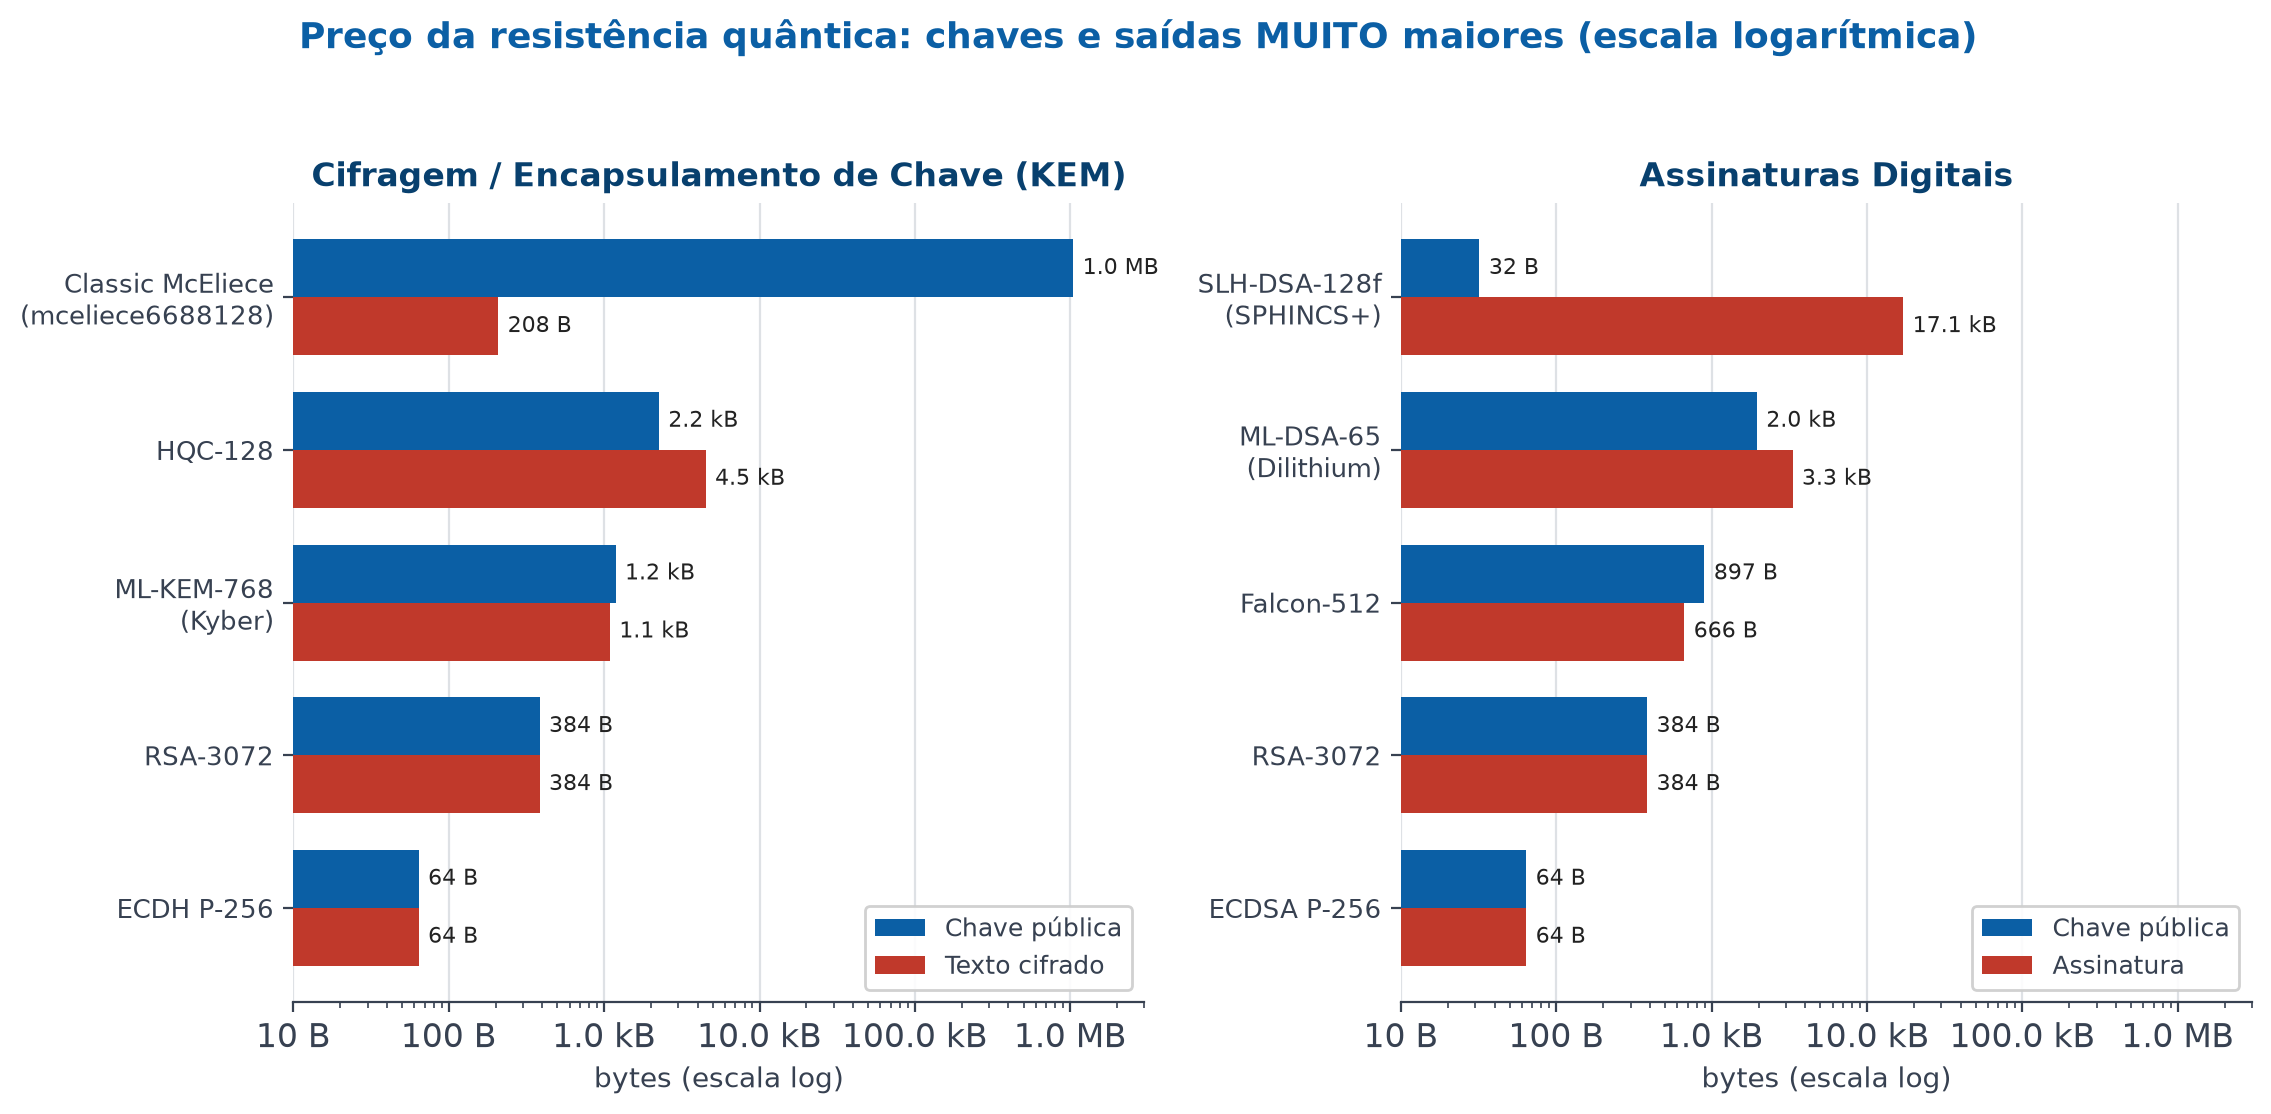
\includegraphics[width=0.88\textwidth]{img/pqc_sizes.png}
    \end{center}
    \vspace{-0.3em}
    \begin{tcolorbox}[colback=blue!5,colframe=blue!50!black,boxrule=0.5pt]
        \footnotesize
        As chaves e saídas são bem maiores que em RSA/ECC (observe a escala logarítmica): o Classic McEliece tem chave de cerca de 1\,MB e o SPHINCS+ tem assinatura de cerca de 17\,kB. Cada família paga o custo em um lugar diferente.
    \end{tcolorbox}
    \smallskip
    {\tiny Tamanhos (bytes) das especificações NIST FIPS 203/204/205 e das submissões (Classic McEliece, HQC, Falcon).}
\end{frame}

%%%%%%%%%%%%%%%%%%%%%%%%%%%%%%%%%%%%%%%%%%%%%%%%%%%%%%%%%%%%%%%%%%%%%
\section{Criptografia Baseada em Reticulados}

\begin{frame}{O que é um Reticulado (\textit{Lattice})}
    Um reticulado é o conjunto de todas as combinações inteiras dos vetores de uma base.
    \begin{center}
        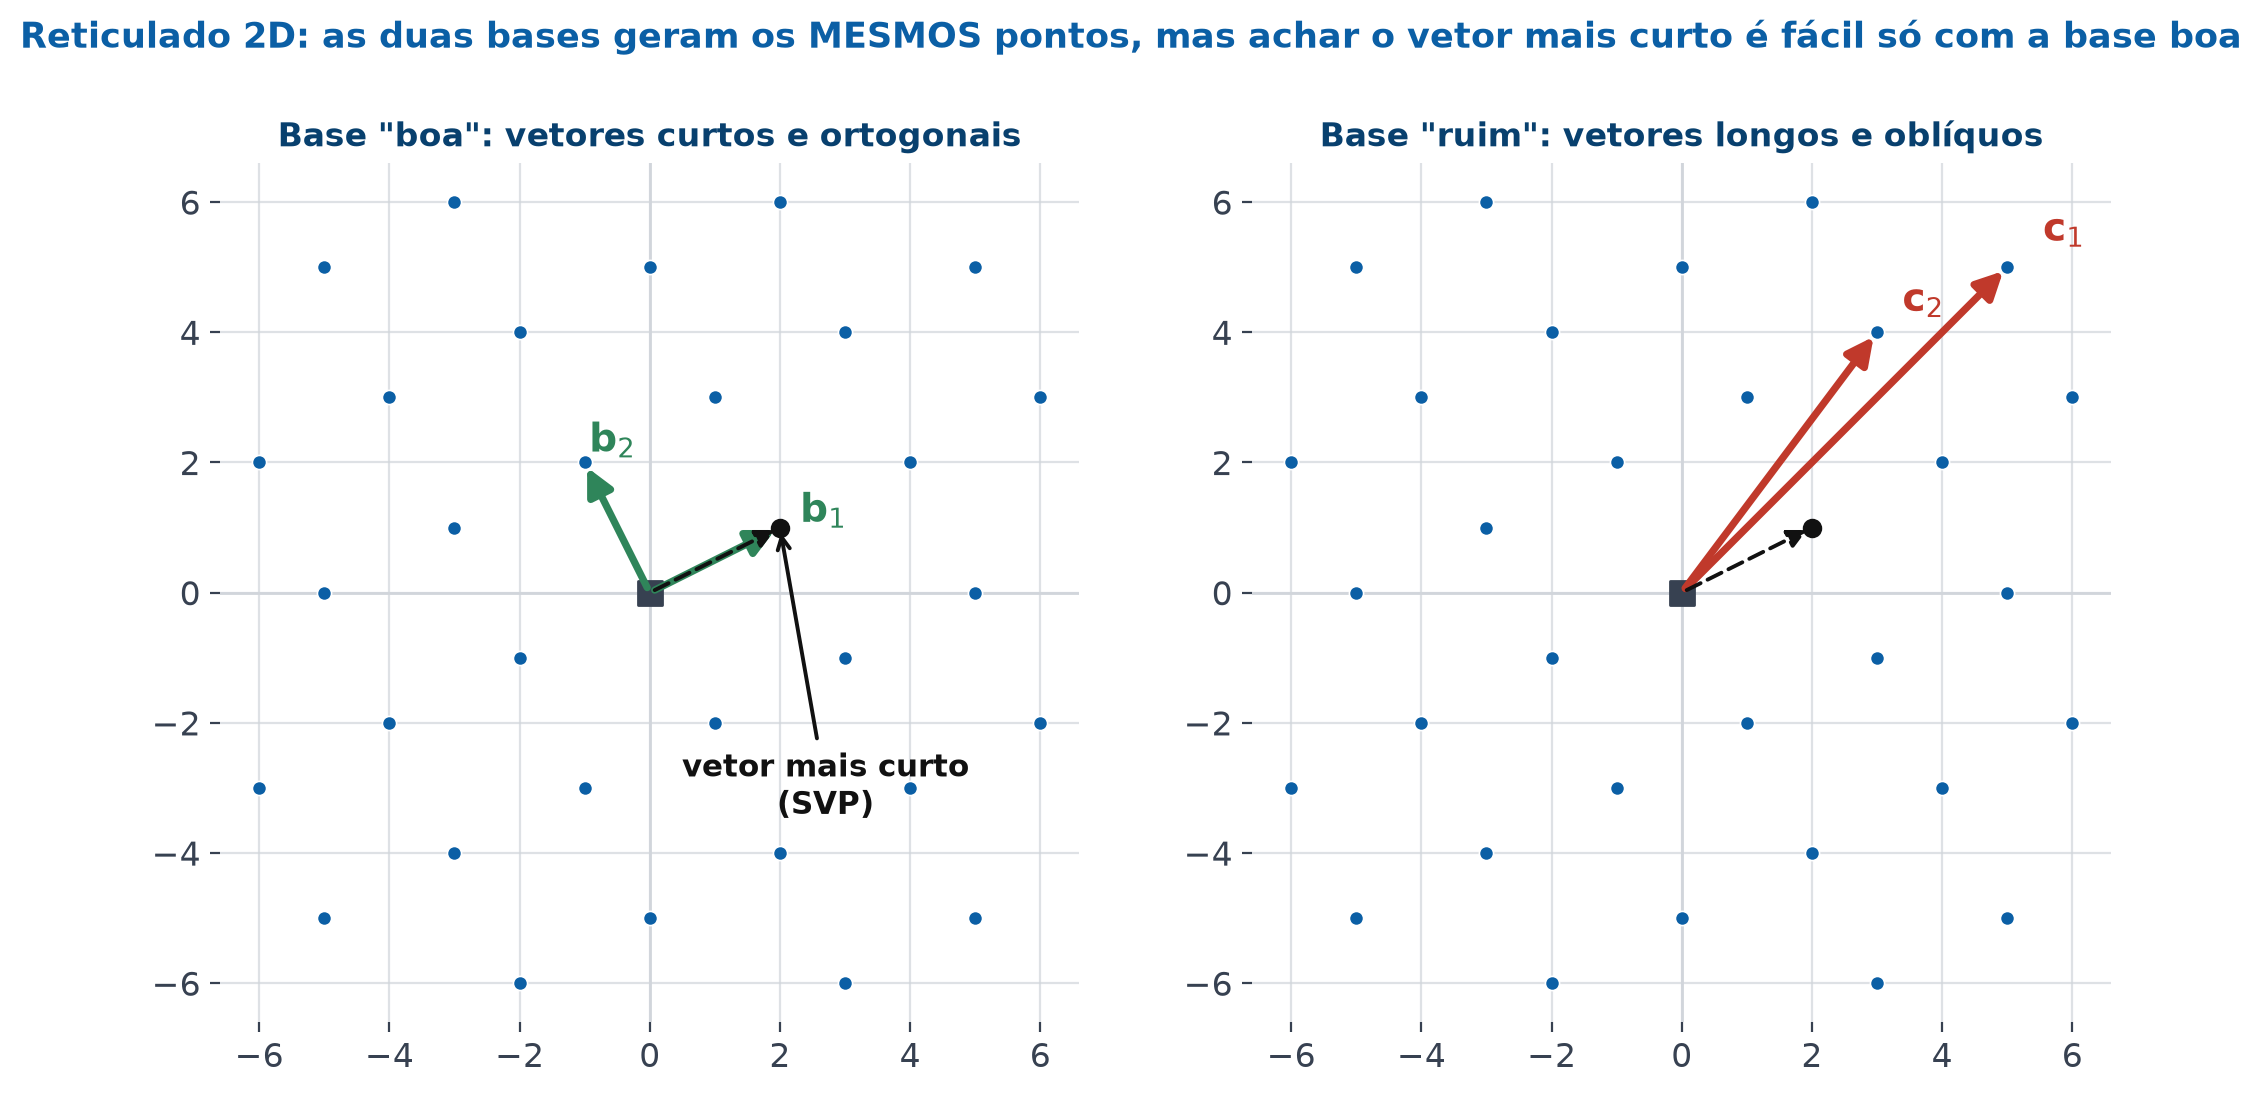
\includegraphics[width=0.72\textwidth]{img/lattice_svp.png}
    \end{center}
    \vspace{-0.3em}
    \begin{tcolorbox}[colback=gray!8,colframe=gray!60!black,boxrule=0.5pt]
        \footnotesize
        \textbf{Problema do Vetor Mais Curto (SVP):} dado o reticulado por uma base ``ruim'', achar o vetor não-nulo mais curto. É fácil em 2D, mas muito difícil em centenas de dimensões, inclusive para computadores quânticos.
    \end{tcolorbox}
    \smallskip
    {\tiny Fonte: Paar et al.\ (2024), §12.2 (reticulados e SVP).}
\end{frame}

\begin{frame}{Learning With Errors (LWE): a Ideia do Ruído}
    O LWE esconde um segredo $\mathbf{s}$ somando um pequeno erro $\mathbf{e}$ a um sistema linear:
    \begin{tcolorbox}[colback=gray!8,colframe=gray!60!black,boxrule=0.5pt]
        \centering\footnotesize
        $\mathbf{b} \equiv A\,\mathbf{s} + \mathbf{e} \pmod{q}$ \qquad ($\mathbf{s}$ secreto; $\mathbf{e}$ = ruído pequeno)
    \end{tcolorbox}
    \smallskip
    {\footnotesize Exemplo ($q = 13$, $\mathbf{s} = (3,1)$); cada linha é $\langle \mathbf{a}_i,\mathbf{s}\rangle + e_i \equiv b_i$:}
    \begin{center}
    \renewcommand{\arraystretch}{1.0}
    \scriptsize
    \begin{tabular}{c c c c}
        \toprule
        $\mathbf{a}_i$ & $\langle \mathbf{a}_i, \mathbf{s}\rangle \bmod 13$ & erro $e_i$ & $b_i$ \\
        \midrule
        $(1,\,2)$ & $5$ & $+1$ & $6$ \\
        $(4,\,1)$ & $0$ & $\phantom{+}0$ & $0$ \\
        $(2,\,3)$ & $9$ & $-1$ & $8$ \\
        $(5,\,5)$ & $7$ & $+1$ & $8$ \\
        \bottomrule
    \end{tabular}
    \end{center}
    \vspace{-0.3em}
    \begin{tcolorbox}[colback=blue!5,colframe=blue!50!black,boxrule=0.5pt]
        \footnotesize
        Com $\mathbf{s}$, cada $\langle \mathbf{a}_i,\mathbf{s}\rangle$ fica \emph{perto} de $b_i$ (só difere pelo erro). Sem ele, tudo parece ruído: recuperar $\mathbf{s}$ é o \textbf{problema LWE}.
    \end{tcolorbox}
    \smallskip
    {\tiny Fonte: Paar et al.\ (2024), §12.2.1 (\textit{Learning With Errors}).}
\end{frame}

\begin{frame}{O Papel do Ruído na Segurança}
    \begin{columns}[T]
        \begin{column}{0.5\textwidth}
            \begin{tcolorbox}[colback=red!5,colframe=red!60!black,boxrule=0.5pt,title={\footnotesize Sem ruído ($\mathbf{e}=0$)}]
                \footnotesize
                $\mathbf{b} = A\mathbf{s}$ é um sistema linear comum.\\[2pt]
                A eliminação de Gauss recupera $\mathbf{s}$ em tempo polinomial. Nenhuma segurança.
            \end{tcolorbox}
        \end{column}
        \begin{column}{0.5\textwidth}
            \begin{tcolorbox}[colback=green!6,colframe=green!50!black,boxrule=0.5pt,title={\footnotesize Com ruído ($\mathbf{e}\neq 0$)}]
                \footnotesize
                Cada equação está ``levemente errada''.\\[2pt]
                Gauss propaga e amplifica o erro; resolver vira uma busca em um reticulado gigante. Difícil.
            \end{tcolorbox}
        \end{column}
    \end{columns}
    \medskip
    \begin{tcolorbox}[colback=gray!8,colframe=gray!60!black,boxrule=0.5pt]
        \footnotesize
        Em dimensões grandes ($n$ de centenas a milhares), recuperar $\mathbf{s}$ equivale a achar um vetor curto no reticulado, o SVP. É essa dificuldade, com redução de segurança ao SVP, que sustenta os esquemas de reticulados.
    \end{tcolorbox}
    \smallskip
    {\scriptsize \textbf{SVP} = \textit{Shortest Vector Problem} (o vetor não-nulo mais curto). \textbf{SIVP} = \textit{Shortest Independent Vectors Problem} (vários vetores independentes curtos). O LWE reduz-se a versões \emph{aproximadas} desses problemas.\par}
    \smallskip
    {\tiny Fonte: Paar et al.\ (2024), §12.2 (redução de LWE ao SVP).}
\end{frame}

\begin{frame}{De LWE aos Padrões: Ring/Module-LWE, Kyber e Dilithium}
    \begin{itemize}
        \footnotesize
        \item O LWE ``puro'' exige matrizes $A$ grandes, logo chaves grandes. A saída é usar estrutura algébrica:
        \begin{itemize}
            \scriptsize
            \item \textbf{Ring-LWE} e \textbf{Module-LWE} usam polinômios em vez de vetores, tornando as chaves bem mais compactas e rápidas.
        \end{itemize}
        \item É sobre Module-LWE que se constroem os principais padrões do NIST:
    \end{itemize}
    \smallskip
    \begin{tcolorbox}[colback=green!6,colframe=green!50!black,boxrule=0.5pt]
        \footnotesize
        \begin{itemize}
            \item \textbf{Kyber}, padronizado como \textbf{ML-KEM} (FIPS 203), para encapsulamento de chave (KEM).
            \item \textbf{Dilithium}, padronizado como \textbf{ML-DSA} (FIPS 204), para assinatura digital.
        \end{itemize}
        \smallskip
        O \textbf{Falcon} (FN-DSA, FIPS 206, em finalização) também é de reticulados, mas com outra estrutura: reticulados \textbf{NTRU} (baseados em anéis de polinômios, de 1996), não Module-LWE.
    \end{tcolorbox}
    \vspace{-0.2em}
    \begin{tcolorbox}[colback=blue!5,colframe=blue!50!black,boxrule=0.5pt]
        \footnotesize
        Os reticulados são a família preferida do NIST: bom equilíbrio entre tamanho e velocidade.
    \end{tcolorbox}
    \vspace{-0.1em}
    {\tiny Fonte: Paar et al.\ (2024), §12.2.3 (Ring-LWE); NIST FIPS 203/204; FIPS 206 (em finalização).}
\end{frame}

%%%%%%%%%%%%%%%%%%%%%%%%%%%%%%%%%%%%%%%%%%%%%%%%%%%%%%%%%%%%%%%%%%%%%
\section{Criptografia Baseada em Códigos}

\begin{frame}{Códigos Corretores de Erro: Revisão Rápida}
    \begin{itemize}
        \footnotesize
        \item Um código corretor adiciona redundância para que erros de transmissão possam ser detectados e corrigidos.
        \item A matriz geradora $G$ codifica a mensagem: $\mathbf{c} = \mathbf{m}\,G$. A matriz de paridade $H$ verifica: a síndrome $\mathbf{s} = H\,\mathbf{c}^{\mathsf T}$ é $\mathbf{0}$ se não há erro.
        \item Se um bit foi corrompido, a síndrome indica qual, no que se chama decodificação por síndrome.
    \end{itemize}
    \medskip
    \begin{tcolorbox}[colback=gray!8,colframe=gray!60!black,boxrule=0.5pt]
        \footnotesize
        \textbf{Ideia de McEliece (1978):} e se, em vez de corrigir erros, usarmos os erros de propósito como parte do segredo? Decodificar um código linear genérico é NP-difícil no pior caso; e decodificar um código que parece aleatório é tido como difícil na prática (caso médio). É nisso que se apoia a segurança.
    \end{tcolorbox}
    \smallskip
    {\tiny Fonte: Paar et al.\ (2024), §12.3.1 (códigos lineares, $G$, $H$, síndrome).}
\end{frame}

\begin{frame}{O Criptossistema de McEliece (1978): a Ideia}
    \footnotesize
    Como em todo sistema de chave pública (RSA, ECC), quem vai \emph{receber} as mensagens monta o par de chaves. Aqui é o \textbf{Bob}. A ideia central: um código corretor só é fácil de decodificar para quem conhece a sua \textbf{estrutura}.
    \medskip
    \begin{itemize}
        \item Bob parte de um código com decodificador eficiente, o \textbf{código Goppa} $G$ (secreto).
        \item Ele o \textbf{embaralha} com duas matrizes secretas e publica $\hat{G} = S\,G\,P$:
        \begin{itemize}\scriptsize
            \item[--] $P$ (\textbf{matriz de permutação}): troca a \emph{ordem das colunas} (as posições), disfarçando a estrutura do código Goppa;
            \item[--] $S$ (\textbf{matriz invertível}): embaralha as \emph{linhas} (a codificação), para que $\hat{G}$ não entregue a mensagem.
        \end{itemize}
        \item \textbf{Chave pública de Bob:} $\hat{G}$. \quad \textbf{Chave privada de Bob:} $G$ (Goppa), $S$ e $P$.
    \end{itemize}
    \smallskip
    \begin{tcolorbox}[colback=blue!5,colframe=blue!50!black,boxrule=0.5pt]
        \footnotesize
        \textbf{Por que duas?} Cada uma esconde uma coisa: sozinha, $P$ deixaria o código ainda \emph{reconhecível}; $S$ sozinha geraria o \emph{mesmo} código (não disfarça nada). Juntas, $\hat{G}$ parece um gerador aleatório, e corrigir erros nele (sem $S$ e $P$) é difícil.
    \end{tcolorbox}
    \smallskip
    {\tiny Fonte: Paar et al.\ (2024), §12.3.2 (McEliece / códigos Goppa).}
\end{frame}

\begin{frame}{McEliece: Alice Cifra, Bob Decifra}
    \footnotesize
    \textbf{Alice} envia a mensagem $\mathbf{m}$ a Bob usando a \textbf{chave pública} $\hat{G}$ dele. Só \textbf{Bob}, com sua \textbf{chave privada} $(S,P)$, consegue decifrar.
    \begin{center}
    \resizebox{0.96\textwidth}{!}{%
    \begin{tikzpicture}[font=\footnotesize, node distance=0.7cm]
        \node[bloco, fill=green!8, draw=green!50!black] (G) {Código \textbf{Goppa} secreto\\(sabe corrigir $t$ erros)};
        \node[bloco, right=1.1cm of G] (scramble) {embaralha:\\ $\hat{G} = S\,G\,P$};
        \node[bloco, fill=blue!8, draw=blue!55!black, right=1.1cm of scramble] (pub) {\textbf{Chave pública} $\hat{G}$\\(Bob publica)};
        \draw[lig] (G) -- (scramble);
        \draw[lig] (scramble) -- (pub);
        % encrypt / decrypt row
        \node[bloco, below=1.2cm of G, fill=orange!10, draw=orange!70!black] (enc) {\textbf{Alice} cifra (usa $\hat{G}$):\\ $\mathbf{y} = \mathbf{m}\hat{G} + \mathbf{e}$\\ (soma $t$ erros de propósito)};
        \node[bloco, below=1.2cm of pub, fill=red!7, draw=red!60!black] (dec) {\textbf{Bob} decifra (usa $S,P$):\\ corrige os $t$ erros com o\\ Goppa e recupera $\mathbf{m}$};
        \draw[lig] (pub) -- (enc);
        \draw[lig] (enc) -- (dec);
    \end{tikzpicture}%
    }
    \end{center}
    \vspace{-0.2em}
    \begin{tcolorbox}[colback=red!5,colframe=red!60!black,boxrule=0.5pt]
        \footnotesize
        \textbf{Oscar} (o atacante) vê apenas $\mathbf{y}$: um código que parece aleatório, com erros somados. Sem $S$ e $P$, remover esses erros é a \textbf{decodificação de síndrome}, um problema difícil.
    \end{tcolorbox}
    \smallskip
    {\tiny Fonte: Paar et al.\ (2024), §12.3.2 (McEliece); §12.3.3 (variante de Niederreiter).}
\end{frame}

\begin{frame}{Por que Códigos de Goppa?}
    \footnotesize
    O McEliece não usa um código qualquer: usa os \textbf{códigos de Goppa}, uma família de códigos lineares definidos por um \textbf{polinômio secreto} sobre um corpo finito. Duas propriedades os tornam ideais:
    \medskip
    \begin{itemize}
        \item \textbf{Decodificação eficiente:} há um algoritmo rápido que corrige até $t$ erros, \emph{desde que} se conheça o polinômio de Goppa. É o que permite a Bob decifrar.
        \item \textbf{Bom disfarce:} embaralhado por $S$ e $P$, um código de Goppa é \emph{difícil de distinguir} de um código linear aleatório. Ninguém sabe recuperar a estrutura a partir de $\hat{G}$.
    \end{itemize}
    \medskip
    \begin{tcolorbox}[colback=red!5,colframe=red!60!black,boxrule=0.5pt]
        \footnotesize
        A escolha do código \textbf{importa}: variantes que trocaram Goppa por códigos com \emph{estrutura demais} (como os Reed--Solomon generalizados) foram \textbf{quebradas}. Os códigos de Goppa resistem a ataques desde \textbf{1978}.
    \end{tcolorbox}
    \smallskip
    {\tiny Fonte: Paar et al.\ (2024), §12.3; V.\ D.\ Goppa (1970); quebra de GRS: Sidelnikov--Shestakov (1992).}
\end{frame}

\begin{frame}{Códigos na Prática: McEliece, BIKE, HQC}
    \begin{itemize}
        \footnotesize
        \item \textbf{Classic McEliece}: quase 50 anos sem ataque prático, o que gera alta confiança. Em compensação, a chave pública é muito grande (cerca de 1\,MB), inviável para muitos cenários.
        \item \textbf{BIKE} e \textbf{HQC}: usam códigos estruturados (quase-cíclicos) para reduzir bastante o tamanho das chaves (cerca de 1 a 5\,kB), ao custo de menos anos de confiança.
    \end{itemize}
    \medskip
    \begin{tcolorbox}[colback=green!6,colframe=green!50!black,boxrule=0.5pt]
        \footnotesize
        \textbf{Novidade (mar/2025):} o NIST selecionou o \textbf{HQC} como KEM adicional baseado em códigos, uma reserva estratégica com base matemática diferente do ML-KEM (reticulados). Se um dia os reticulados forem quebrados, o HQC continua disponível.
    \end{tcolorbox}
    \medskip
    \begin{tcolorbox}[colback=blue!5,colframe=blue!50!black,boxrule=0.5pt]
        \footnotesize
        A criptografia baseada em códigos serve bem para KEM, mas a expansão de chave e texto cifrado a torna ruim para cifrar grandes volumes diretamente.
    \end{tcolorbox}
    \smallskip
    {\tiny Fonte: Paar et al.\ (2024), §12.3.4 (Classic McEliece, BIKE); NIST (seleção do HQC, mar/2025).}
\end{frame}

%%%%%%%%%%%%%%%%%%%%%%%%%%%%%%%%%%%%%%%%%%%%%%%%%%%%%%%%%%%%%%%%%%%%%
\section{Criptografia Baseada em Hash}

\begin{frame}{Assinaturas a Partir Apenas de Funções Hash}
    \begin{tcolorbox}[colback=green!6,colframe=green!50!black,boxrule=0.5pt]
        \footnotesize
        É a família mais conservadora: sua segurança depende apenas da resistência de uma função hash (que já sabemos ser quântico-resistente com saída grande), sem suposições matemáticas novas.
    \end{tcolorbox}
    \medskip
    \begin{itemize}
        \footnotesize
        \item Limitação: serve apenas para assinaturas, não para KEM.
        \item A construção é feita em camadas: primeiro a assinatura de uso único (OTS), depois o Winternitz (mais compacto) e por fim a árvore de Merkle (para muitos usos).
    \end{itemize}
    \medskip
    \begin{tcolorbox}[colback=blue!5,colframe=blue!50!black,boxrule=0.5pt]
        \footnotesize
        É a base do \textbf{SPHINCS+}, padronizado como \textbf{SLH-DSA} (FIPS 205): uma assinatura sem estado (\textit{stateless}), lenta e volumosa, porém com a maior margem de confiança.
    \end{tcolorbox}
    \smallskip
    {\tiny Fonte: Paar et al.\ (2024), §12.4; NIST FIPS 205 (SLH-DSA).}
\end{frame}

\begin{frame}{Assinatura de Uso Único de Lamport (LD-OTS)}
    A chave privada são $2n$ valores \textbf{aleatórios} (um par por bit); a pública são as \textbf{imagens} deles por uma função de mão única $f$. Assina-se revelando a pré-imagem de cada bit.
    \vspace{0.2em}
    {\footnotesize Exemplo com $f(x) = x^2 \bmod 253$ (função de Rabin, $253 = 11 \cdot 23$), mensagem de 3 bits:}
    \begin{center}
    \renewcommand{\arraystretch}{1.0}
    \scriptsize
    \begin{tabular}{c c c}
        \toprule
        \textbf{bit} & \textbf{chave privada} $(x_{i,0},\,x_{i,1})$ & \textbf{chave pública} $(f(x_{i,0}),\,f(x_{i,1}))$ \\
        \midrule
        0 & $(17,\ 23)$ & $(36,\ 23)$ \\
        1 & $(31,\ 45)$ & $(202,\ 1)$ \\
        2 & $(9,\ 50)$ & $(81,\ 223)$ \\
        \bottomrule
    \end{tabular}
    \end{center}
    \vspace{-0.5em}
    \begin{tcolorbox}[colback=blue!5,colframe=blue!50!black,boxrule=0.5pt]
        \footnotesize
        Para assinar $\mathbf{m} = (1,0,1)$, revele $(x_{0,1},\,x_{1,0},\,x_{2,1}) = (23,\,31,\,50)$.\\
        \textbf{Verificação:} $f(23)=23$, $f(31)=202$, $f(50)=223$, que batem com a chave pública nas posições dos bits. \checkmark
    \end{tcolorbox}
    \vspace{-0.5em}
    \begin{tcolorbox}[colback=red!5,colframe=red!60!black,boxrule=0.5pt]
        \footnotesize
        \textbf{Uso único:} assinar duas mensagens com a mesma chave revela pré-imagens demais e permite falsificação. Cada par de chaves serve para uma assinatura.
    \end{tcolorbox}
    \smallskip
    {\tiny Fonte: Paar et al.\ (2024), §12.4.1 (Lamport--Diffie OTS).}
\end{frame}

\begin{frame}{Winternitz e a Árvore de Merkle}
    \begin{itemize}
        \footnotesize
        \item \textbf{Winternitz (W-OTS)}: em vez de um par por bit, assina blocos de $w$ bits aplicando $f$ repetidamente (cadeias de hash). Troca tamanho por tempo: assinaturas menores, com mais aplicações de hash.
        \item OTS e W-OTS ainda são de uso único. Para assinar muitas mensagens sem publicar milhares de chaves públicas, usamos uma árvore de Merkle.
    \end{itemize}
    \medskip
    \begin{tcolorbox}[colback=gray!8,colframe=gray!60!black,boxrule=0.5pt]
        \footnotesize
        \textbf{Árvore de Merkle (MSS):} as $2^{t}$ chaves públicas de uso único são combinadas, hash a hash, em uma única raiz. Essa raiz é a chave pública de todas elas.
    \end{tcolorbox}
    \smallskip
    {\tiny Fonte: Paar et al.\ (2024), §12.4.1 (Winternitz) e §12.4.2 (Merkle Signature Scheme).}
\end{frame}

\begin{frame}{Árvore de Merkle: Uma Chave Pública para $2^t$ Assinaturas}
    \begin{center}
    \resizebox{0.70\textwidth}{!}{%
    \begin{tikzpicture}[font=\footnotesize, level distance=1.0cm,
        level 1/.style={sibling distance=5.2cm},
        level 2/.style={sibling distance=2.6cm}]
        \node[raiz] (root) {raiz $=$ \textbf{chave pública}}
            child {node[noh] (n0) {$h(\cdot\,\|\,\cdot)$}
                child {node[folha] {$Y_0$}}
                child {node[folha] {$Y_1$}}}
            child {node[noh] (n1) {$h(\cdot\,\|\,\cdot)$}
                child {node[folha] {$Y_2$}}
                child {node[folha] {$Y_3$}}};
        \node[align=center, font=\scriptsize, text=black!60] at (0,-3.4)
            {folhas $Y_i = $ chaves públicas de uso único (OTS)};
    \end{tikzpicture}%
    }
    \end{center}
    \vspace{-0.3em}
    \begin{tcolorbox}[colback=green!6,colframe=green!50!black,boxrule=0.5pt]
        \footnotesize
        Para assinar com $Y_i$, envie a assinatura OTS junto com os nós irmãos no caminho até a raiz (o caminho de autenticação). O verificador recomputa a raiz e a compara com a chave pública.
    \end{tcolorbox}
    \vspace{-0.1em}
    {\footnotesize \textbf{Escala:} uma altura $t=20$ dá $2^{20} \approx$ 1 milhão de assinaturas com uma só chave pública. É preciso lembrar quais folhas já foram usadas (esquema com estado).}
    \smallskip
    {\tiny Fonte: Paar et al.\ (2024), §12.4.2 (MSS, caminho de autenticação, raiz como chave pública).}
\end{frame}

%%%%%%%%%%%%%%%%%%%%%%%%%%%%%%%%%%%%%%%%%%%%%%%%%%%%%%%%%%%%%%%%%%%%%
\section{A Fronteira e Lições de Humildade}

\begin{frame}{Propostas que Foram Quebradas}
    A PQC é uma área jovem e sob criptoanálise ativa. Dois casos recentes mostram por quê:
    \medskip
    \begin{tcolorbox}[colback=red!5,colframe=red!60!black,boxrule=0.5pt,title={\footnotesize Multivariada (Rainbow)}]
        \footnotesize
        Finalista do NIST em assinaturas multivariadas, foi quebrada em 2022: um ataque recuperava a chave em um fim de semana num laptop.
    \end{tcolorbox}
    \medskip
    \begin{tcolorbox}[colback=red!5,colframe=red!60!black,boxrule=0.5pt,title={\footnotesize Isogenias (SIKE)}]
        \footnotesize
        Candidato promissor, com chaves pequenas, foi quebrado em 2022 por um ataque matemático clássico, que sequer precisou de computador quântico.
    \end{tcolorbox}
    \medskip
    \begin{tcolorbox}[colback=blue!5,colframe=blue!50!black,boxrule=0.5pt]
        \footnotesize
        \textbf{Lição:} a confiança em criptografia vem de anos de tentativas de ataque. Por isso o processo do NIST é aberto e demorado, e por isso se mantém um portfólio de famílias (reticulados, códigos e hash).
    \end{tcolorbox}
\end{frame}

\begin{frame}{Agilidade Criptográfica e Hibridização}
    \begin{tcolorbox}[colback=green!6,colframe=green!50!black,boxrule=0.5pt,title={\footnotesize Agilidade criptográfica (\textit{crypto-agility})}]
        \footnotesize
        Projetar sistemas de modo a trocar de algoritmo sem reescrever tudo. Se um esquema cair, é possível substituí-lo rapidamente, como seria necessário caso os reticulados fossem quebrados.
    \end{tcolorbox}
    \medskip
    \begin{tcolorbox}[colback=blue!5,colframe=blue!50!black,boxrule=0.5pt,title={\footnotesize Abordagem híbrida}]
        \footnotesize
        Durante a transição, rodar clássico e pós-quântico ao mesmo tempo (por exemplo, ECDH e ML-KEM). A chave só é comprometida se ambos forem quebrados, o que protege contra falhas na PQC nova e contra o computador quântico.
    \end{tcolorbox}
    \medskip
    {\footnotesize Veremos adiante que o híbrido é a estratégia oficial de várias potências e já está em produção na internet.}
    \smallskip
    {\tiny Fonte: Paar et al.\ (2024), §12.5--12.6; orientações NIST/BSI/ANSSI.}
\end{frame}

%%%%%%%%%%%%%%%%%%%%%%%%%%%%%%%%%%%%%%%%%%%%%%%%%%%%%%%%%%%%%%%%%%%%%
\section{Padronização pelo NIST}

\begin{frame}{O Processo de Padronização do NIST}
    \begin{center}
        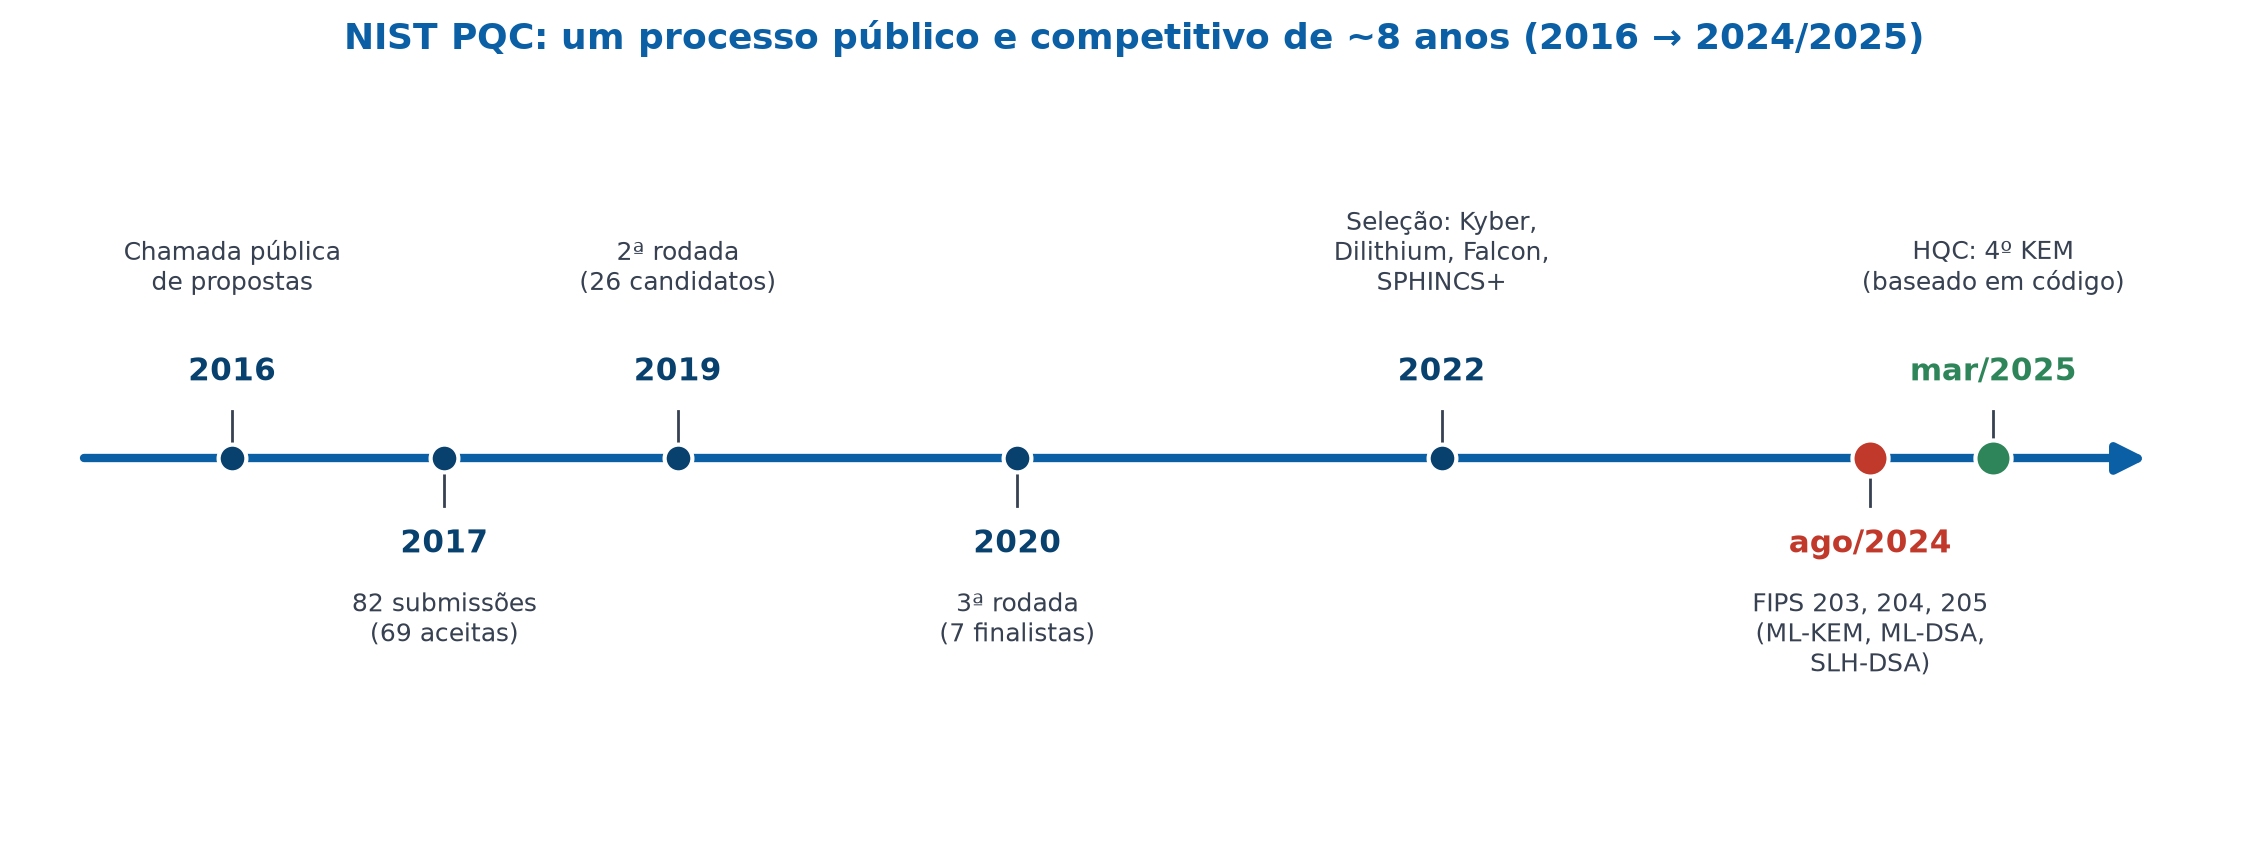
\includegraphics[width=0.99\textwidth]{img/nist_process_timeline.png}
    \end{center}
    \vspace{-0.2em}
    \begin{tcolorbox}[colback=blue!5,colframe=blue!50!black,boxrule=0.5pt]
        \footnotesize
        Em 2016 o NIST abriu uma chamada pública mundial. Após três rodadas de análise e criptoanálise aberta, selecionou os vencedores em 2022 e publicou os padrões finais em agosto de 2024.
    \end{tcolorbox}
    \smallskip
    {\tiny Fonte: NIST PQC Standardization Project (csrc.nist.gov/projects/post-quantum-cryptography).}
\end{frame}

\begin{frame}{Os Padrões Finais do NIST (2024--2025)}
    \begin{center}
    \renewcommand{\arraystretch}{1.3}
    \scriptsize
    \begin{tabularx}{\linewidth}{@{}l l l >{\raggedright\arraybackslash}X@{}}
        \toprule
        \textbf{Padrão} & \textbf{Nome (algoritmo)} & \textbf{Base matemática} & \textbf{Função} \\
        \midrule
        \rowcolor{blue!7} \textbf{FIPS 203} & ML-KEM (Kyber) & Reticulados (Module-LWE) & Encapsulamento de chave \\
        \rowcolor{blue!7} \textbf{FIPS 204} & ML-DSA (Dilithium) & Reticulados (Module-LWE) & Assinatura digital \\
        \rowcolor{green!7} \textbf{FIPS 205} & SLH-DSA (SPHINCS+) & Funções hash & Assinatura digital \\
        \textbf{FIPS 206} & FN-DSA (Falcon) & Reticulados (NTRU) & Assinatura compacta \emph{(em finalização)} \\
        \rowcolor{orange!10} \textbf{(HQC)} & HQC & Códigos & KEM adicional \emph{(mar/2025)} \\
        \bottomrule
    \end{tabularx}
    \end{center}
    \medskip
    \begin{tcolorbox}[colback=green!6,colframe=green!50!black,boxrule=0.5pt]
        \footnotesize
        Dois pilares para o dia a dia: \textbf{ML-KEM} (trocar chaves) e \textbf{ML-DSA} (assinar). \textbf{SLH-DSA} e \textbf{HQC} são as reservas conservadoras, com matemática independente dos reticulados.
    \end{tcolorbox}
    \smallskip
    {\tiny Fonte: NIST FIPS 203, 204, 205 (ago/2024); FIPS 206 (rascunho); seleção do HQC (mar/2025).}
\end{frame}

%%%%%%%%%%%%%%%%%%%%%%%%%%%%%%%%%%%%%%%%%%%%%%%%%%%%%%%%%%%%%%%%%%%%%
\section{Comparação entre Potências Globais}

\begin{frame}{Por que a Soberania Criptográfica Importa}
    \begin{itemize}
        \footnotesize
        \item A criptografia é infraestrutura estratégica: quem define o padrão influencia a segurança (e a vigilância) global.
        \item Após décadas confiando em padrões dos EUA (NIST), várias potências passaram a desenvolver os seus próprios, por soberania e por desconfiança de possíveis \textit{backdoors}.
    \end{itemize}
    \medskip
    \begin{tcolorbox}[colback=blue!5,colframe=blue!50!black,boxrule=0.5pt]
        \footnotesize
        \textbf{Tensão central:} há convergência (quase todos migram até cerca de 2030 a 2035, por causa do \textit{harvest now, decrypt later}) e, ao mesmo tempo, divergência (padrões e filosofias diferentes, o que gera desafios de interoperabilidade).
    \end{tcolorbox}
    \medskip
    {\footnotesize A seguir, como EUA, União Europeia, Reino Unido, China e Rússia estão conduzindo a transição.}
\end{frame}

\begin{frame}{Panorama Comparativo dos Padrões Pós-Quânticos}
    \begin{center}
    \renewcommand{\arraystretch}{1.35}
    \tiny
    \begin{tabularx}{\linewidth}{@{}l l >{\raggedright\arraybackslash}X >{\raggedright\arraybackslash}X l@{}}
        \toprule
        \textbf{Potência} & \textbf{Agência} & \textbf{Padrões / estratégia} & \textbf{Postura híbrida} & \textbf{Prazo} \\
        \midrule
        \rowcolor{blue!7} \textbf{EUA} & NIST / NSA & FIPS 203/204/205 (+HQC, +Falcon); CNSA 2.0 & NSA prefere \textbf{PQC puro} nos sistemas nacionais & 2030--2035 \\
        \textbf{Alemanha} & BSI & ML-KEM \textbf{+ FrodoKEM + Classic McEliece} (reservas) & \textbf{Híbrido obrigatório} & 2030 / 2032 \\
        \rowcolor{green!7} \textbf{França} & ANSSI & Padrões NIST, em 3 fases & \textbf{Híbrido} em KEM e assinatura & cert.\ 2027 \\
        \textbf{Reino Unido} & NCSC & Padrões NIST & Híbrido na transição & 2028/31/35 \\
        \rowcolor{red!7} \textbf{China} & ICCS (sob a OSCCA) & \textbf{Competição própria} (2025); reticulados ``não-estruturados'' & em definição & $\sim$2028 (padrões) \\
        \textbf{Rússia} & TC26 & Sucessores \textbf{PQ do GOST} & em definição & $\sim$2030+ \\
        \bottomrule
    \end{tabularx}
    \end{center}
    \vspace{-0.2em}
    \begin{tcolorbox}[colback=gray!8,colframe=gray!60!black,boxrule=0.5pt]
        \footnotesize
        \textbf{Contraste marcante:} os EUA (NSA) não exigem híbrido para sistemas nacionais, enquanto a Alemanha (BSI) e a França (ANSSI) o exigem, numa postura mais conservadora.
    \end{tcolorbox}
    \smallskip
    {\tiny Fontes: NIST FIPS 203--205; NSA CNSA 2.0; BSI TR-02102-1; ANSSI; UK NCSC; ICCS/OSCCA; Rússia TC26.}
\end{frame}

\begin{frame}{Prazos de Migração: EUA, UE, Reino Unido, China, Rússia}
    \begin{center}
        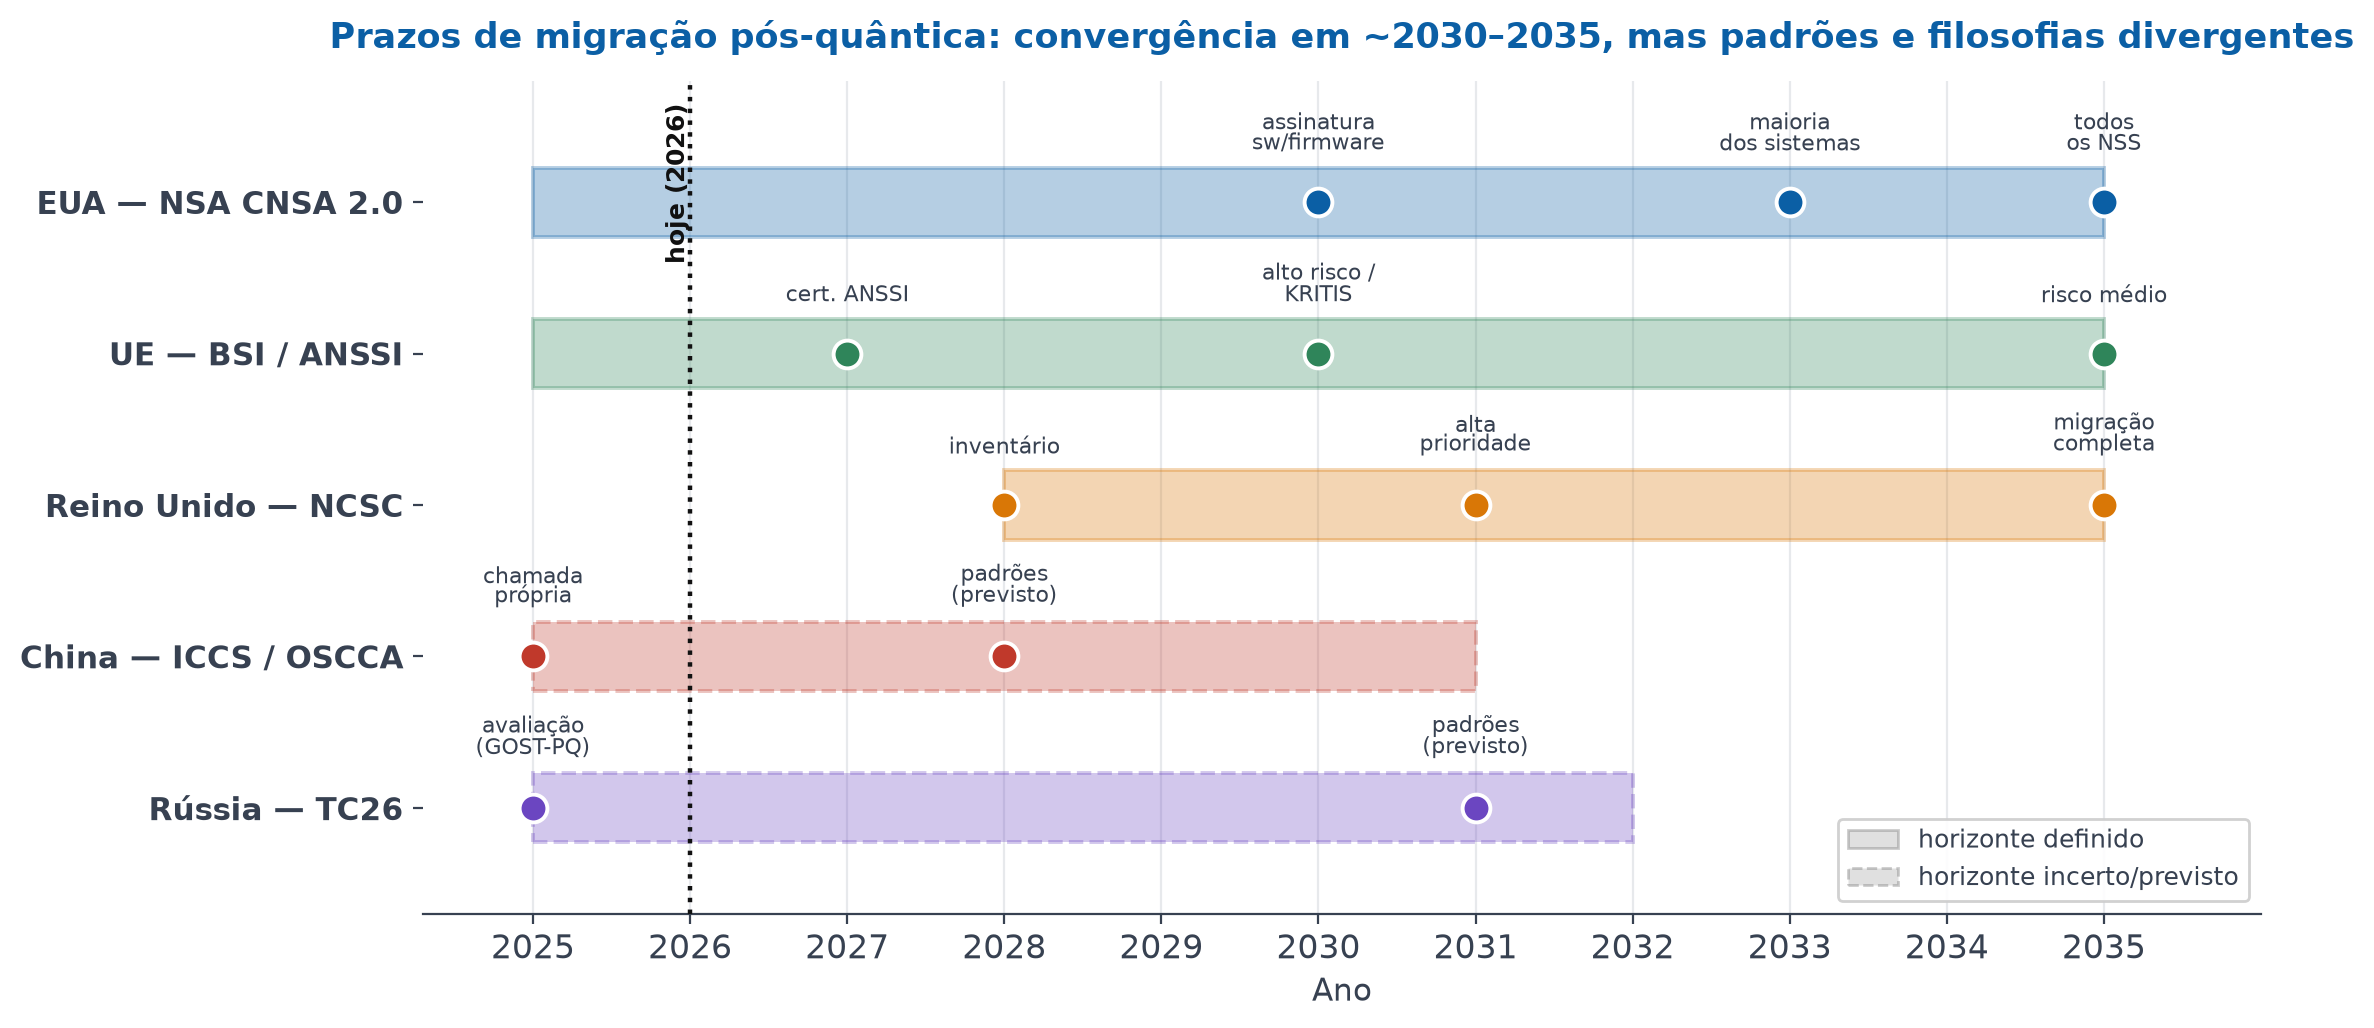
\includegraphics[width=0.95\textwidth]{img/global_pqc_timeline.png}
    \end{center}
    \vspace{-0.5em}
    \begin{tcolorbox}[colback=blue!5,colframe=blue!50!black,boxrule=0.5pt]
        \footnotesize
        A convergência gira em torno de 2030 a 2035: a \textbf{NSA CNSA 2.0} (EUA) até 2035; a \textbf{UE} (declaração conjunta BSI/ANSSI e mais 17 estados) protege o mais sensível até 2030; o \textbf{NCSC} (UK) em 2028, 2031 e 2035. China e Rússia ainda trabalham com prazos estimados.
    \end{tcolorbox}
    \smallskip
    {\tiny Fontes: NSA CNSA 2.0; roadmap coordenado da UE + BSI/ANSSI; UK NCSC (\textit{Timelines for migration to PQC}, 2025).}
\end{frame}

\begin{frame}{Divergências de Filosofia e o Resto do Mundo}
    \begin{itemize}
        \footnotesize
        \item \textbf{China (ICCS, sob a OSCCA):} lançou em fev/2025 uma competição própria (cifra, assinatura, hash e cifra de bloco), preferindo reticulados ``não-estruturados'' aos reticulados algébricos do NIST. Já possui a família clássica SM2/SM3/SM4/SM9. A motivação declarada é a soberania e a independência tecnológica.
        \item \textbf{Rússia (TC26):} avalia sucessores quântico-resistentes do GOST (assinatura GOST R 34.10, hash Streebog, cifra Kuznyechik) por meio de um centro nacional criado em 2022. O processo é pouco transparente e controla a importação de criptografia estrangeira.
    \end{itemize}
    \medskip
    \begin{tcolorbox}[colback=gray!8,colframe=gray!60!black,boxrule=0.5pt]
        \footnotesize
        \textbf{E os demais?} Japão (CRYPTREC), Coreia do Sul (competição KpqC), Canadá (CSE) e Austrália (ASD) também têm roteiros. Os padrões ISO/IEC devem harmonizar parte disso, mas a fragmentação é real.
    \end{tcolorbox}
    \smallskip
    {\tiny Fontes: ICCS/OSCCA (chamada 2025); Rússia TC26 / Academia de Criptografia; CRYPTREC; KpqC; CSE; ASD; ISO/IEC JTC 1/SC 27.}
\end{frame}

%%%%%%%%%%%%%%%%%%%%%%%%%%%%%%%%%%%%%%%%%%%%%%%%%%%%%%%%%%%%%%%%%%%%%
\section{Migração na Prática}

\begin{frame}{Migração Híbrida na Prática: TLS 1.3 com ML-KEM}
    A internet já está migrando: a troca de chaves do TLS combina o ECDH clássico com o ML-KEM.
    \vspace{0.2em}
    \begin{center}
    \resizebox{0.9\textwidth}{!}{%
    \begin{tikzpicture}[font=\footnotesize]
        \node[ator] (A) at (0,0) {Cliente};
        \node[ator] (B) at (10,0) {Servidor};
        \foreach \x in {0,10} \draw[vida] (\x,-0.85) -- (\x,-5.2);
        \draw[msg] (0,-1.4) -- (10,-1.4)
            node[rotmsg, midway]{ClientHello: chave X25519 \textbf{+} chave ML-KEM-768};
        \node[comp, anchor=north] at (10,-1.75) {responde X25519 \textbf{+} encapsula ML-KEM};
        \draw[msg] (10,-3.0) -- (0,-3.0)
            node[rotmsg, midway]{ServerHello: resposta X25519 \textbf{+} ciphertext ML-KEM};
        \node[comp, anchor=north] at (0,-3.35) {segredo $=$ KDF(\,ss$_{\text{X25519}}$ $\,\|\,$ ss$_{\text{ML-KEM}}$\,)};
        \node[comp, anchor=north] at (10,-3.35) {mesmo segredo combinado};
        \draw[msg] (0,-4.7) -- (10,-4.7) node[rotmsg, midway]{tráfego cifrado (AES-GCM)};
    \end{tikzpicture}%
    }
    \end{center}
    \vspace{-0.2em}
    \begin{tcolorbox}[colback=green!6,colframe=green!50!black,boxrule=0.5pt]
        \footnotesize
        Já em produção: Chrome, Firefox, Cloudflare, AWS e o Signal (protocolo PQXDH) usam trocas de chave híbridas. O segredo permanece seguro se pelo menos um dos dois resistir.
    \end{tcolorbox}
    \smallskip
    {\tiny Fonte: IETF (TLS hybrid key exchange); implantações Google/Cloudflare/AWS/Signal (2023--2026).}
\end{frame}

\begin{frame}{Como Migrar na Prática}
    \begin{enumerate}
        \footnotesize
        \item \textbf{Inventário criptográfico:} descobrir onde e quais algoritmos são usados (bibliotecas, protocolos, certificados, dispositivos). Não é possível migrar o que não se conhece.
        \medskip
        \item \textbf{Priorização:} começar pelo que tem maior prazo de sigilo e maior exposição (dados de longa duração, VPNs, raízes de confiança), guiado pela desigualdade de Mosca.
        \medskip
        \item \textbf{Agilidade criptográfica:} adotar o híbrido onde possível e projetar sistemas que troquem de algoritmo facilmente no futuro.
    \end{enumerate}
    \medskip
    \begin{tcolorbox}[colback=red!5,colframe=red!60!black,boxrule=0.5pt]
        \footnotesize
        Começar cedo é essencial: migrações criptográficas de larga escala levam anos. Como o \textit{harvest now, decrypt later} já está em curso, esperar o CRQC surgir significa começar tarde demais.
    \end{tcolorbox}
    \smallskip
    {\tiny Fonte: NIST SP 1800-38 (\textit{Migration to Post-Quantum Cryptography}); NCSC / ENISA (roteiros de migração).}
\end{frame}

%%%%%%%%%%%%%%%%%%%%%%%%%%%%%%%%%%%%%%%%%%%%%%%%%%%%%%%%%%%%%%%%%%%%%
\section{Conclusão}

\begin{frame}{Lições Aprendidas}
    \begin{itemize}
        \item Quando existir um computador quântico relevante (CRQC), RSA, DH e ECC caem (Shor); a criptografia simétrica e as funções hash apenas dobram parâmetros (Grover).
        \medskip
        \item A PQC são esquemas clássicos (em software) resistentes a ataque quântico. Não confundir com QKD.
        \medskip
        \item Há três famílias maduras, cada uma com seu compromisso: reticulados (equilibrada, preferida), códigos (chaves grandes, muita confiança) e hash (só assinatura, a mais conservadora).
        \medskip
        \item O NIST padronizou ML-KEM, ML-DSA e SLH-DSA (2024), e o HQC (2025). As potências divergem na filosofia (híbrido, soberania), mas convergem no prazo (cerca de 2030 a 2035).
        \medskip
        \item Por causa do ``colher agora, decifrar depois'', a migração (híbrida e com agilidade) é urgente, e não uma preocupação para o futuro distante.
    \end{itemize}
\end{frame}

\begin{frame}{Referências}
    \scriptsize
    \textbf{Livro-texto}
    \begin{itemize}
        \item C. Paar, J. Pelzl, T. Güneysu. \textit{Understanding Cryptography: From Established Symmetric and Asymmetric Ciphers to Post-Quantum Algorithms}. 2.\ ed., Springer, 2024. \textbf{Cap.\ 12} (\textit{Post-Quantum Cryptography}), §§12.1 a 12.6.
    \end{itemize}
    \smallskip
    \textbf{Publicações e projetos do NIST}
    \begin{itemize}
        \item NIST \textbf{FIPS 203} (ML-KEM), \textbf{FIPS 204} (ML-DSA), \textbf{FIPS 205} (SLH-DSA), ago/2024; \textbf{FIPS 206} (FN-DSA, rascunho).
        \item NIST IR 8105 (\textit{Report on Post-Quantum Cryptography}); NIST SP 1800-38 (\textit{Migration to PQC}).
        \item NIST PQC Standardization Project; seleção do \textbf{HQC} (mar/2025). \url{https://csrc.nist.gov/projects/post-quantum-cryptography}
    \end{itemize}
    \smallskip
    \textbf{Agências e potências}
    \begin{itemize}
        \item \textbf{NSA:} CNSA 2.0 (\textit{Commercial National Security Algorithm Suite 2.0}); FAQ sobre QKD.
        \item \textbf{BSI} (Alemanha): TR-02102-1. \textbf{ANSSI} (França): \textit{views on PQC transition}. \textbf{NCSC} (Reino Unido): \textit{Timelines for migration to PQC} (2025).
        \item \textbf{China:} ICCS/OSCCA (chamada de 2025). \textbf{Rússia:} TC26 / Academia de Criptografia. ENISA; ISO/IEC JTC 1/SC 27.
    \end{itemize}
    \smallskip
    {\tiny Definições e prazos traduzidos das fontes primárias; algoritmos de Shor (1994) e Grover (1996); desigualdade de Mosca (2015/2018).}
\end{frame}

\end{document}
